\chapter{Implementation}

\section{Github}

The code for this \gls{poc} is available on Github \cite{github}

\section{Development}

Substrate uses a smart contract language called ink! \cite{ink}. This is basically rust with the standard
library taken away and extensive use of the type system and macros to create an eDSL \cite{edsl}.

The first thing I wanted to model is how we could store \gls{cdm}'s on the blockchain.
We want to be sure we fulfill the following requirements

\begin{enumerate}
    \item We can maintain a table of valid \acrshort{ca} providers and that only the owner of the contract can add 
        providers.
    \item Only a valid \acrshort{ca} provider can add a \gls{cdm}
\end{enumerate}

I modelled a simplified \gls{cdm} as a rust struct see listing \ref{cdm}

\begin{lstlisting}[label={cdm},language=c,caption={CDM Struct}]
pub struct ConjunctionDataMessage {
    pub object1_norad_id: i32,
    pub object2_norad_id: i32,
    pub collision_probabilty: f32,
    pub time_of_closest_pass: i32
}
\end{lstlisting}

ink! \cite{ink} has the concept of storage. This is what we will use for persistance. It's also a struct and you can only create one
in a smart contract. In listing \ref{storage} we have a Vector to store our \gls{cdm}'s and another Vector
to hold the Accounts which are allowed to add \gls{cdm}'s to the storage.


Accounts in Substrate are public addresses. 

\begin{lstlisting}[label={storage},language=c,caption={ink! storage}]
#[ink(storage)]
pub struct Negotiate {
    contract_owner: AccountId,
    cdms: StorageVec<ConjunctionDataMessage>,
    ca_providers: StorageVec<AccountId>
}
\end{lstlisting}

A function on our contract to add a CA provider looks like listing \ref{add_provider}. 
Substrate makes sure that the caller has a corerct mesahe signed by their private key before calling our function. 
We can then check the caller is the contract owner and if so, we add the provider account to our list.

The entry will be stored in the immutable log by all the nodes. So here we have implemented role based access control, 
data integrity and non repudiation. 


\begin{lstlisting}[label={add_provider},language=c,caption={Add a provider}]
pub fn add_ca_provider(&mut self, 
    provider_account: AccountId) {
    // Only the owner of this smart contract can call this.
    assert_eq!(self.env().caller(), self.env().account_id());

    // Add this account to our list of roviders
    self.ca_providers.push(provider_account);
}
\end{lstlisting}

\section{Unit testing}

\section{Local Integration testing}

I was able to get a test node up and running in VSCode \pageref{node}. 
However I wan't able to get the web based client to attach to my node \pageref{canvas}.

\begin{figure}[h]
    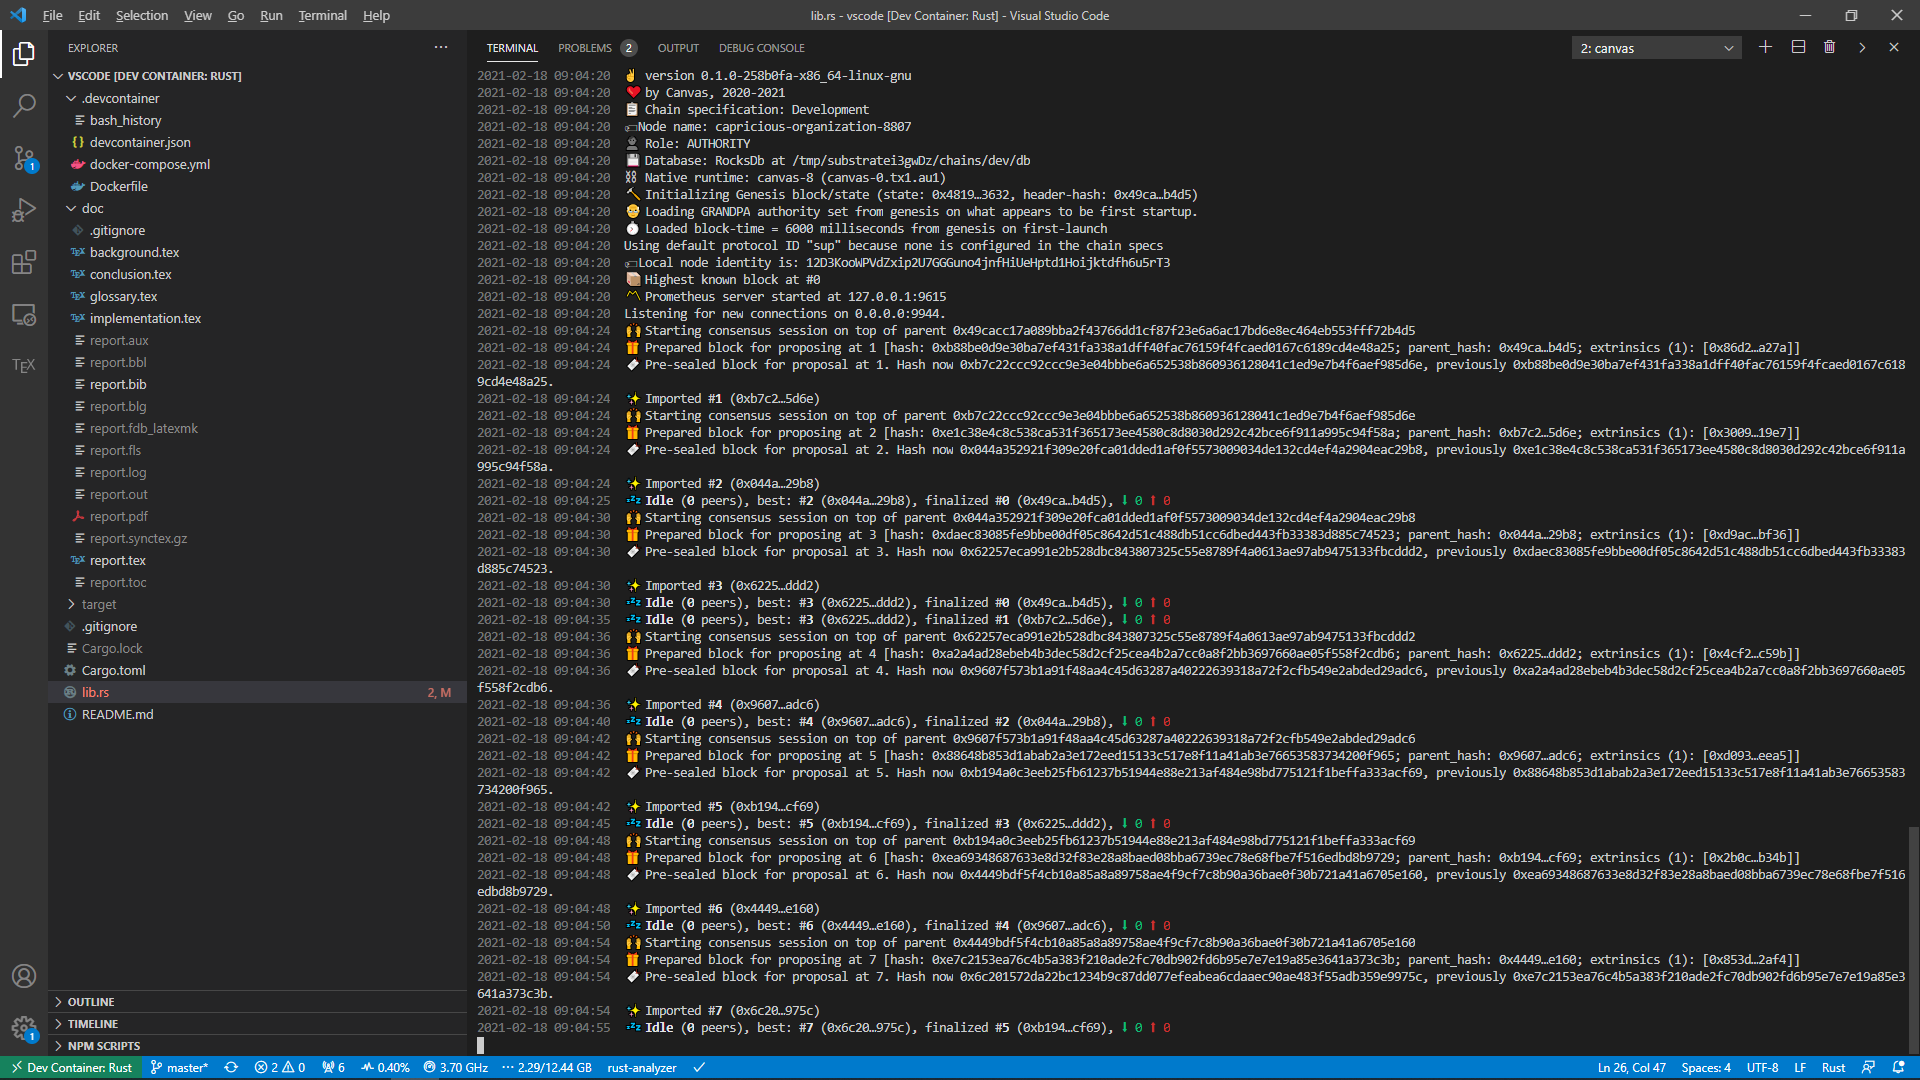
\includegraphics[width=\textwidth]{node-screenshot} 
    \caption{Substrate node running in VSCode terminal}
    \label{node}
\end{figure}

I would require more time to get my contract deployed and tested on a local node.

\begin{figure}[h]
    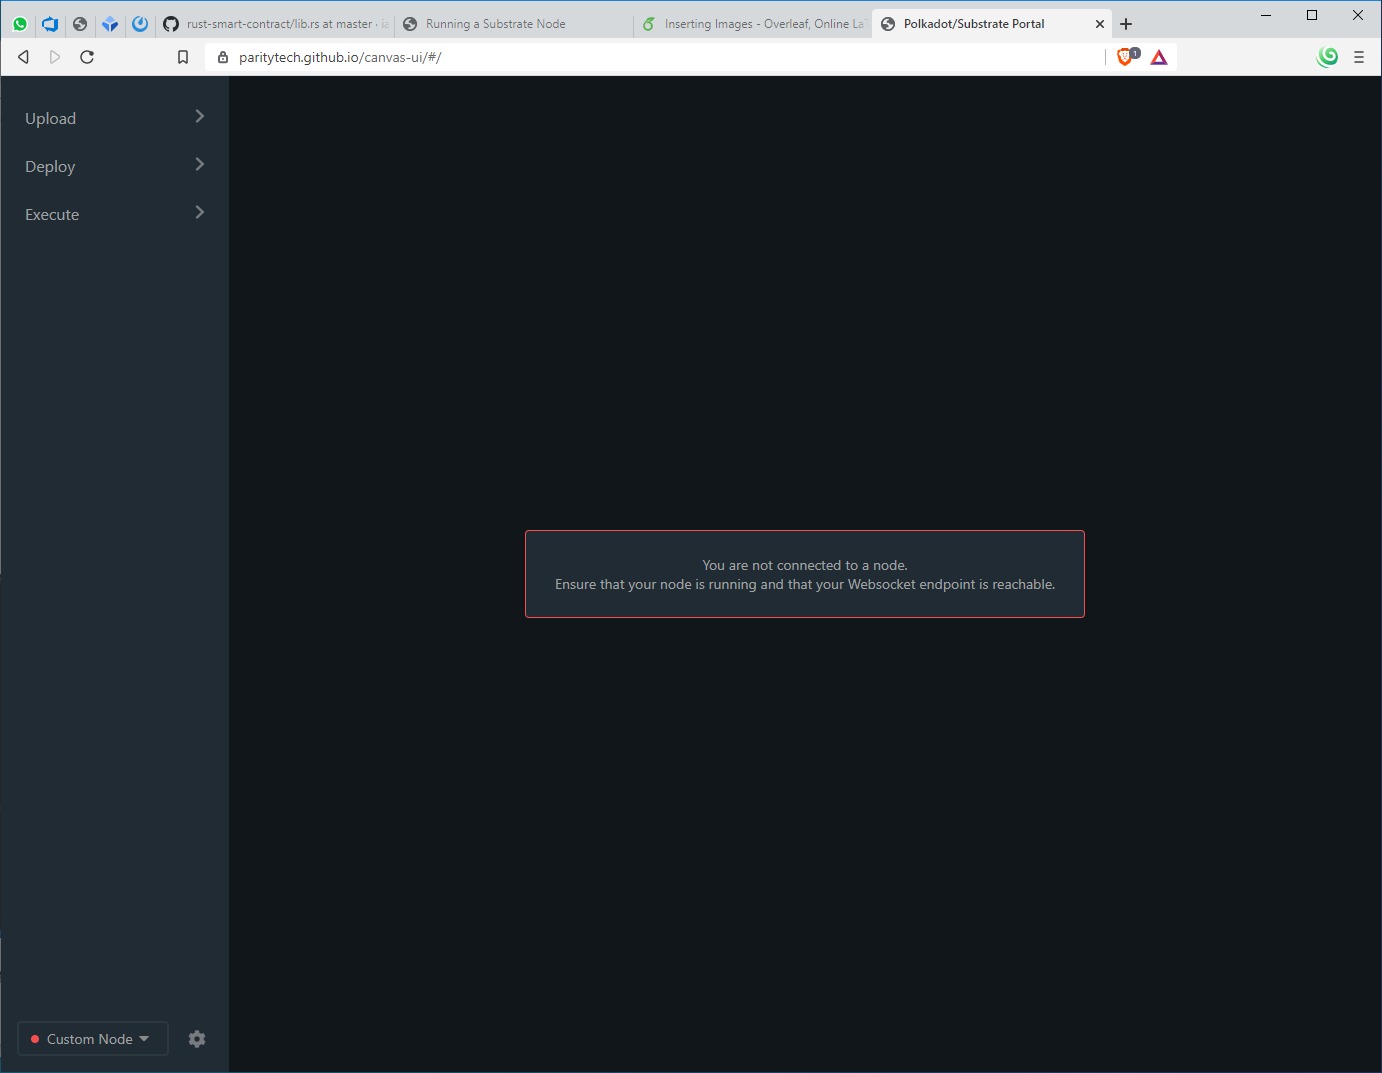
\includegraphics[width=\textwidth]{canvas-ui} 
    \caption{You are not connected to a node}
    \label{canvas}
\end{figure}